\chapter{\label{CH:challenges}Challenges in data reduction. Etalon Cavity Map.}

\section{\label{eta_corr_susec: etalon_transmission}Etalon transmission profile}

The intensity distribution observed at the focal plane of any etalon-based instrument tuned to a wavelength $\lambda_s$ obeys the following expression \citep{franI}:

\begin{multline}
    I\left(\xi, \eta ; \lambda_{s}\right)=g(\xi, \eta)\int_{0}^{\infty} T(\lambda) \iint  O\left(\xi_0, \eta_0 ; \lambda\right) \\ S\left(\xi_0, \eta_0; \xi , \eta; \lambda-\lambda_{s}\right)  \mathrm{d} \xi_{0} \mathrm{~d} \eta_{0}\mathrm{d} \lambda ,
    \label{eq_eta_corr: General}
\end{multline}
where $\xi, \eta$ are the coordinates in the image plane, $T(\lambda)$ accounts for the presence of an order-sorting pre-filter, $O\left(\xi_0, \eta_0 ; \lambda\right)$ represents the brightness distribution of the observed object at the point $\left(\xi_0, \eta_0\right)$, and $S\left(\xi_0, \eta_0; \xi , \eta; \lambda-\lambda_{s}\right)$ accounts for the imaging response of the instrument when tuned at the wavelength $\lambda_{s}$. The latter coincides with the point spread function (PSF) of the instrument when the optical response is invariant against translations. In such a case, we can substitute the last two integrals by the convolution operator, but this is not strictly true in etalon-based instruments, where the response varies pixel to pixel either because of etalon irregularities or because of variations in the illumination across its clear aperture. We have included a new parameter, $g(\xi, \eta)$, that does not appear in the original work by \cite{franI} since pixel-to-pixel differences in the detectors' sensitivity are not considered in the original expression. Therefore, $g(\xi, \eta)$ represents a spatial gain factor that accounts for these wavelength independent pixel-to-pixel intensity fluctuations occurring in the focal plane.

As a first approximation, we assumed a spatial dependence of the imaging response in the form of a Dirac delta in order to simplify the equations. If we let the imaging response follow the expression 
\begin{equation}
S\left(\xi_0, \eta_0; \xi , \eta; \lambda-\lambda_{s}\right)=\delta(\xi_0-\xi,\eta_0-\eta)\Psi(\xi,\eta,\lambda-\lambda_s),
\end{equation}
where $\Psi\left(\xi, \eta ; \lambda-\lambda_{0}\right) $ is the transmission profile of the etalon, Eq. \eqref{eq_eta_corr: General} can be simplified as
\begin{equation}
    I\left(\xi, \eta ; \lambda_{s}\right)=g(\xi, \eta)\int_{0}^{\infty} T(\lambda)  O\left(\xi, \eta ; \lambda\right) \Psi\left(\xi, \eta ; \lambda-\lambda_{s}\right)  \mathrm{d} \lambda.
    \label{eq_eta_corr: intensity}
\end{equation}
The transmission profile has a spatial dependence across the image that arises naturally from the different illumination of the etalon across the FoV in the collimated configuration and from the direct mapping of the local inhomogeneities into the detector in the telecentric configuration. 

Although, in practice, it is not often possible to fully characterize the pre-filter, we assumed it has a rectangular shape centered at the wavelength of the observed spectral line ($\lambda _ {0}$) and a width of $2\Delta \lambda$ such that only one order of the etalon passes through. We note that including a different shape of the pre-filter in the current model is straightforward, provided it can be modeled analytically or even numerically. With this consideration, equation \eqref{eq_eta_corr: intensity} can be written as follows:

\begin{equation}
    I(\xi, \eta ; \lambda_{s})=g(\xi, \eta)\int_{\lambda _{0} - \Delta \lambda}^{\lambda _ {0} + \Delta \lambda}  O(\xi, \eta ; \lambda)  \Psi(\xi, \eta ; \lambda-\lambda_{s})  \mathrm{d} \lambda .
    \label{eq_eta_corr: Intensity-final}
\end{equation}

The explicit shape of $\Psi$  is different depending on the optical configuration of the instrument, that is, collimated or telecentric.
\subsection{One device, two configurations}

file:///home/pablo/Downloads/s10509-023-04212-3.pdf

\subsubsection{\label{eta_corr_susec: collimated}Collimated configuration}

Collimated mounts are characterized by having the etalon located at the pupil plane and therefore receive a collimated beam from each point of the observed object. In this setup, light coming from any point of the object will fall upon the same area of the etalon. Consequently, any local defects on the etalon crystals or on the plates' parallelism is averaged all over the clear aperture, thus making the optical quality constant along the FoV. However, the angle of incidence of the light beam varies along the FoV, thus shifting the transmission profile.  

 The transmission profile for an ideal collimated etalon tuned at wavelength $\lambda _ s$ takes the following form:
\begin{equation}
\Psi ^{\lambda _ s} (\lambda, \theta) = \frac{1}{1 + F \sin ^2 a_s (\lambda,\theta) },
\end{equation}
where
\begin{equation}
a_s (\lambda, \theta) =\frac{2  \pi}{\lambda} nd\cos \theta  \ ,
\label{eq_eta_corr: a-def}
\end{equation}
with the subscript $s$ indicating that the etalon is tuned at the wavelength $\lambda_s$.

The shape of the transmission profile depends on its physical properties. Firstly, the width of the resonance peaks is determined by the parameter $F$, $F \equiv 4R (1 - R )^{-2}$, which depends exclusively on the reflectivity $R$ of its mirrors. Secondly, the spectral behavior of the transmission profile is governed by $a_s(\lambda,\theta)$, which is a function of the refractive index of the etalon cavity, $n$; the distance between mirrors, $d$; and the angle of the incident beam, $\theta$. 

Local defects in the collimated configuration are averaged out, which means that $d$ and $n$ respectively represent the mean values of the thickness and refractive index across the clear aperture of the FPI. Yet, they produce a broadening of the transmission profile and worsen the optical quality of the instrument. The differing angles of incidence over the FoV produce shifts of the transmission that vary quadratically with $\theta$.

\subsubsection{\label{eta_corr_susec: Tele-perfe}Telecentric configuration}

In the telecentric configuration, the etalon is placed very close to an intermediate focal plane, while the pupil is focused at infinity. This way, the etalon is illuminated by cones of rays that are parallel to each other and reach different sections of the interferometer. Local inhomogeneities (defects or cavities) on the etalon produce differences in the transmission profile across the FoV, which are directly mapped into the image plane. This means that the optical response and the transmission profile shift locally on the image sensor. 

The transmission profile of the etalon tuned at a wavelength $\lambda _s $ is, in this case, given by \citep{franIV}:
\begin{equation}
\Psi ^{\lambda _ s} (\lambda) =  \mathfrak{Re}\left[E(a_s (\lambda, n, d, \theta), b) \right] ^2 + \mathfrak{Im}\left[E(a_s(\lambda, n, d, \theta), b) \right] ^2 ,
\label{Eqn: Tel_first}
\end{equation}
with $E(a,b)$ being:
\begin{multline}
E(a, b) = 2 \sqrt{\tau}\ \Biggl\{ \int_0^1 \frac{\varrho \cos \left(a\left[1-b \varrho^2\right]\right)}{1+F \sin ^2\left(a\left[1-b \varrho^2\right]\right)} \mathrm{d} \varrho \ + \\
\mathrm{i} \frac{1+R}{1-R} \int_0^1 \frac{\varrho \sin \left(a\left[1-b \varrho^2\right]\right)}{1+F+ \sin ^2\left(a\left[1-b \varrho^2\right]\right)} \mathrm{d} \varrho\Biggr\} ,
\end{multline}
where $\tau$ is the transmission factor of the etalon at normal incidence, $\varrho$ is the radial coordinate of the pupil normalized to the pupil radius of the instrument, $a$ is defined by Eq. \eqref{eq_eta_corr: a-def} and $b$ is given by
\begin{equation}
b = \frac{1}{8 (nf\#) ^2}.
\end{equation}

This parameter accounts for the contribution of the focal ratio, $f\#$, and has an impact on the spectral resolution and the apodization of the pupil as seen from the etalon \citep{beckers}. Thus, the resolution is now affected by both $F$ and $f\#$, through the parameters $a$ and $b$.

Contrary to the collimated case, $a$ now has an explicit dependence on the spatial coordinates of the image plane, as $n$ and $d$ change from pixel to pixel. These variations compose the "cavity error" of the etalon and need to be corrected when employing telecentric configurations.

\subsubsection{\label{eta_corr_susec: Tele-imperfe}Telecentric imperfect configuration}
The equations shown in Sect.~\ref{eta_corr_susec: Tele-perfe} are valid whenever the incident cone of rays is perpendicular to the etalon mirrors. We refer to this situation hereinafter as "perfect telecentrism". However, real instruments are likely to present deviations from such an ideal case. These deviations can be caused by an intentional tilt of the etalon to suppress ghost images on the detector \citep{ghosts-etalon}, by an accidental tilted angle of incidence caused by deviations from the ideal paraxial propagation of rays within the instrument, or simply because of misalignment of the optical components. In the three cases, the incident cone of rays is no longer perpendicular to the etalon, and hence, we consider these scenarios to have imperfections in the telecentrism degree. One important consequence of the loss of telecentrism is an asymmetrization of the transmission profile that must be accounted for when modeling the instrument response.

The transmission profile in this case is influenced by the angle of incidence of the chief ray at each point of the clear aperture of the etalon, in addition to the parameters mentioned in the previous sections. Unfortunately, the equations for the transmission profile in these configurations are much more complicated than in the ideal telecentric case, with no analytical solution to the integrals of the transmission profile. The integrals and their corresponding derivatives can only be obtained via numerical methods \citep{franI}. 
\begin{figure}
    \centering
    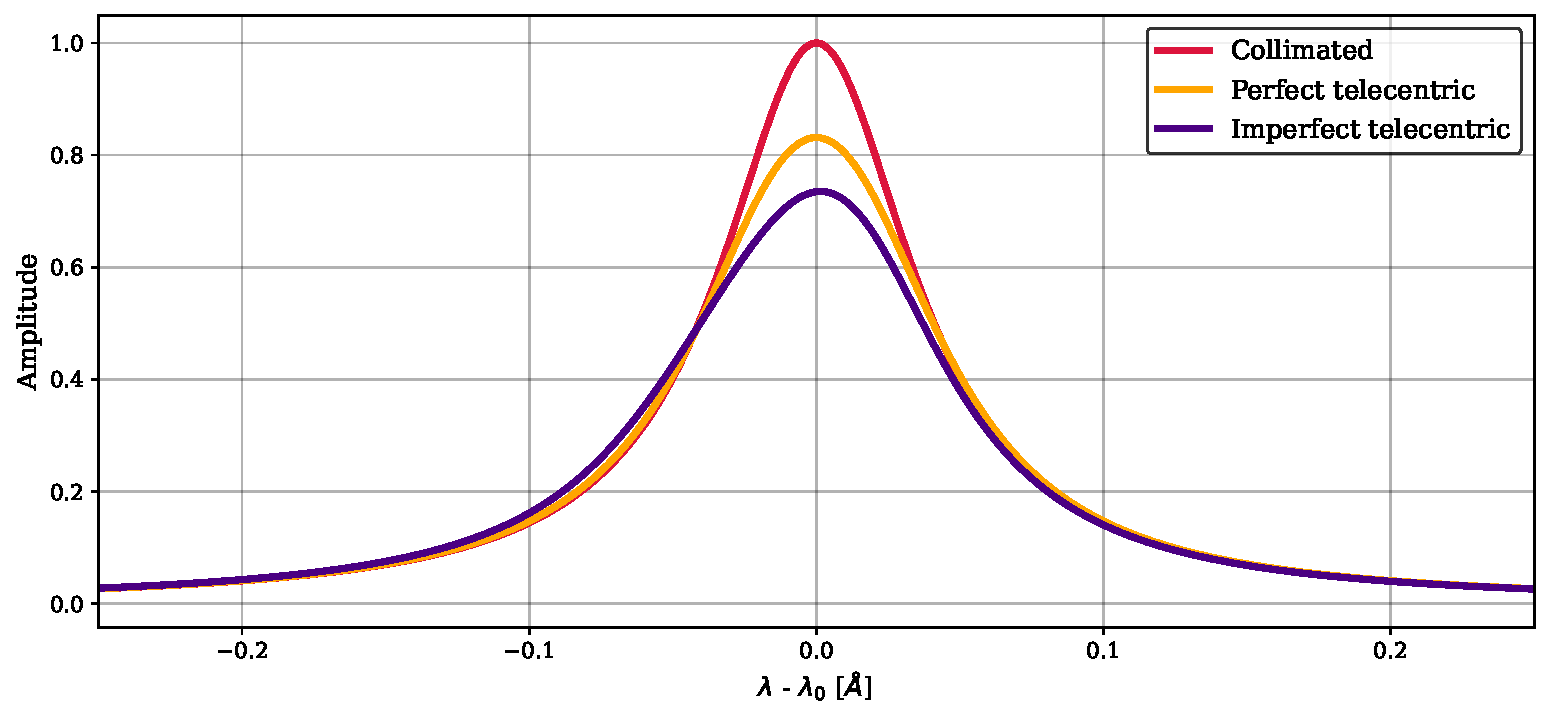
\includegraphics[width = \textwidth]{figures/EtalonPaper/etalon_setups_profiles.pdf}
    \caption{Central peak of the etalon's transmission profile for the three different configurations. The parameters of the etalon are $R = 0.92$, $n = 2.29$, $d = 251 \, \mu \mathrm{m}$, $f\#=56$, $\theta = 0 ^{\circ}$ (collimated and perfect telecentric), and $\Theta = 0.3\,^{\circ}$ (imperfect telecentric)}
    \label{fig_etalon:Profiles-configs}
\end{figure}
Figure \ref{fig_etalon:Profiles-configs} shows the transmission profile corresponding to the three different scenarios we have considered: collimated illumination of the etalon, perfect telecentrism, and imperfect telecentrism. The etalon parameters have been selected to coincide with those of SO/PHI's etalon. In both the collimated and perfect telecentric configurations, a normal incidence  ($\theta = 0$) scenario is shown, whereas in the imperfect telecentric case, we assumed an angle of incidence of the chief ray, $\Theta$, of $0.3^{\circ}$. The parameter $a$ has been adjusted slightly in order to tune the transmission profile at $\lambda _ 0$.

We observed that the telecentric configurations achieve lower peak transmissions than the collimated case. In addition, the telecentric profiles are wider due to the different incidence angles across the illuminating cone of rays. Such a broadening increases with decreasing f-ratios. Lastly, non-normal incidence of the chief ray in the telecentric configuration further widens and shifts ($\sim 4$~m\r{A}
for $\Theta=0.3^\circ$) the profile, making it asymmetrical. 

\subsection{\label{eta_corr_susec: simulating obs} Simulated observations}
  
All the instruments built around the use of an etalon as a wavelength filtering element operate in a very similar way. They scan a spectral line by tuning the etalon (by changing the distance between mirrors and/or modifying the refractive index) to a desired number of wavelengths along the spectral line. At each spectral position, the solar scene is recorded. The measured intensity is approximately given by Eq.~\eqref{eq_eta_corr: Intensity-final}, with the etalon's transmission profile centered at the desired wavelength.

We carried out a series of simulations of a spectral line observation in different conditions. We used the Kitt Peak FTS-Spectral-Atlas as the reference \citep{fts} and, specifically, the Fe I spectral line at 6173.3~\r{A}. Each observation was composed of $N_\lambda$ wavelengths, where the measured intensity was recorded. At every wavelength $\lambda_s$, the corresponding transmission profile of the etalon $\Psi^{\lambda_s}$ was computed, and the "observed" intensity $I ^{\lambda _ s} _ {{\rm obs}, i}$ corresponding to a specific spatial location $(\xi, \eta)$, represented hereinafter by the pixel $i$, was calculated using Eq.~\eqref{eq_eta_corr: Intensity-final}. Additionally, we took into account the presence of additive Gaussian noise. This noise does not necessarily respond to any parameter fluctuation within our analytical expressions or photon noise but comes from any unexpected variations that may not have been modeled in the theoretical scheme.

Additionally, we included the presence of defects arising from irregularities or inhomogeneities on either the cavity thickness $d$, the refractive index $n$, or from deviations of the angle of incidence $\theta$. In order to simulate this, we introduced a relative perturbation $\Delta a$ into the etalon equation that accounts for any local deviation of the value of $a$ with respect to its nominal value. This parameter changes from pixel to pixel differently for the collimated and telecentric configurations. In the former, the profile shifts across the FoV only because of the different incidence angles of the light beam on the etalon. In the latter, local variations of $n$ and/or $d$ are mapped directly onto the detector. We also note that variations in the incidence angle must be considered as well when the degree of telecentrism varies along the detector. Analytically, the parameter $a$ at each $i$-th pixel is given by $a' _ i = a \Delta a _ i$, where $a = (2\pi/\lambda) n d\cos\theta$ is constant along the FoV.

We let $n _ i ^{\lambda_s}$ be the  noise contribution at the $i$-th pixel and wavelength $\lambda_s$. Thus, the observed intensity at that pixel when the etalon is tuned at $\lambda _s$, $I ^{\lambda _ s} _ {{\rm obs}, i}$ is given by 
\begin{equation}
I ^{\lambda _ s} _ {{\rm obs}, i} = g_i \frac{\int_{\lambda_0 - \Delta \lambda}^{\lambda_0 + \Delta \lambda} O(\lambda)\Psi^{\lambda _ s} (\lambda , \Delta a _i)  d\lambda}{\int_{\lambda_0 - \Delta \lambda}^{\lambda_0 + \Delta \lambda} O(\lambda)\Psi^{\lambda _ c} (\lambda, \Delta a _ i)  d\lambda} + n _ i ^{\lambda_s}    ,
\label{eq: Profile - General}
\end{equation}
with $\lambda _ c$ being the continuum wavelength. From a practical point of view, the integration limits are set in such a way that only a single resonance (or order) of the etalon is included with the limits, thus, acting akin to the sorting pre-filter commented on previously. We note that the denominator strictly corresponds to the intensity at the continuum of the line in the absence of the transmission profile or if the continuum wavelength is far enough from the spectral line. In any other case, the transmission should be taken into account as well to normalize the observations to the local continuum, which is necessary since we work with relative measurements. An example of a spectral line measurement is displayed in Fig.~\ref{fig_etalon_corr: Prof-Measure}.
\begin{figure}
    \centering
    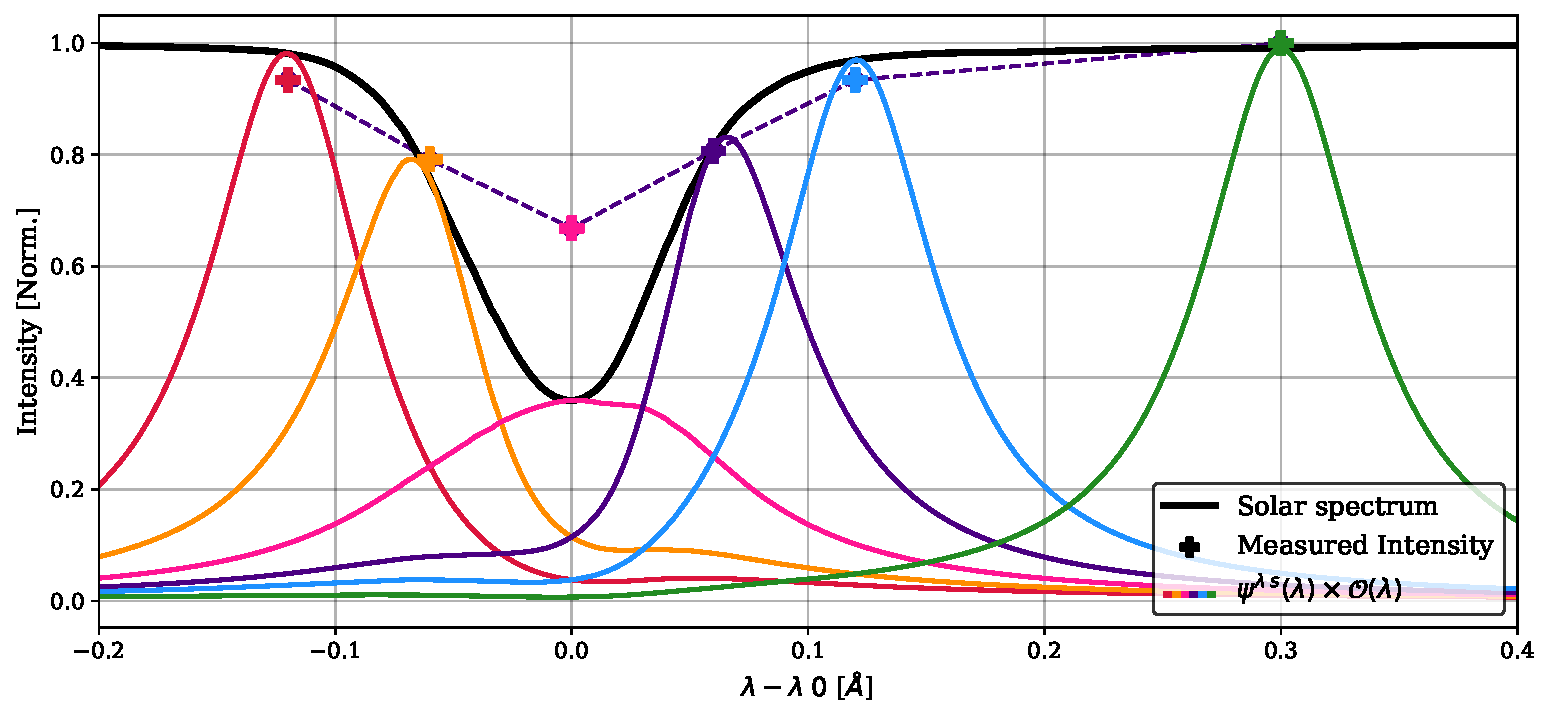
\includegraphics[width = \textwidth]{figures/EtalonPaper/ProfileMeasurement.pdf}
    \caption{Simulated observation of the Fe I spectral line ($\lambda _ 0 = 6173.3$\r{A}) using a collimated mount and a total of $N_ \lambda = 6$ wavelengths that have been equally distributed along the spectral line, with the exception of the continuum measurement (light blue), which is selected at $300$ m\r{A} from the blue of the line core. The measured intensity is the result of computing the value given by Eq.~\ref{eq: Profile - General} at each wavelength and with $g = 1$.
    } \label{fig_etalon_corr: Prof-Measure}
\end{figure}

For both the collimated and telecentric configurations, we modeled etalon and gain imperfections over a $100\times100$~px$^2$ image. Pixel-to-pixel variations in the sensor efficiency were modeled following a random spatial distribution, as shown in Fig.~ \ref{fig_etalon_corr: Inputs} (top panel). Additionally, we included a set of pixels with very low gain values, which represent a group of dead pixels or dust grains.

We modeled the etalon defects as changes in $\Delta a$ in such a way that the maximum displacement reaches $3$ pm. The spatial distribution of the values of  $\Delta a $ follows an increasing radial distribution, as shown in Fig.~ \ref{fig_etalon_corr: Inputs} (bottom panel). Such a spatial distribution coincides with the expected one in collimated etalons due to the change in the incidence angle across the FoV. Telecentric mounts do not exhibit a spatial distribution of their defects such as this, but using the same spatial distribution in the two cases allowed us to compare the performance of the method for both setups in a systematic way. Since $\Delta a$ accounts for relative perturbations, it is by definition an adimensional parameter. However, to grant it a physical meaning, we express the values of $\Delta a$ in \r{A}, representing the associated shift of the transmission profile with respect to the original position determined by $a$.

\begin{figure}
    \begin{minipage}[c]{0.5\textwidth}
        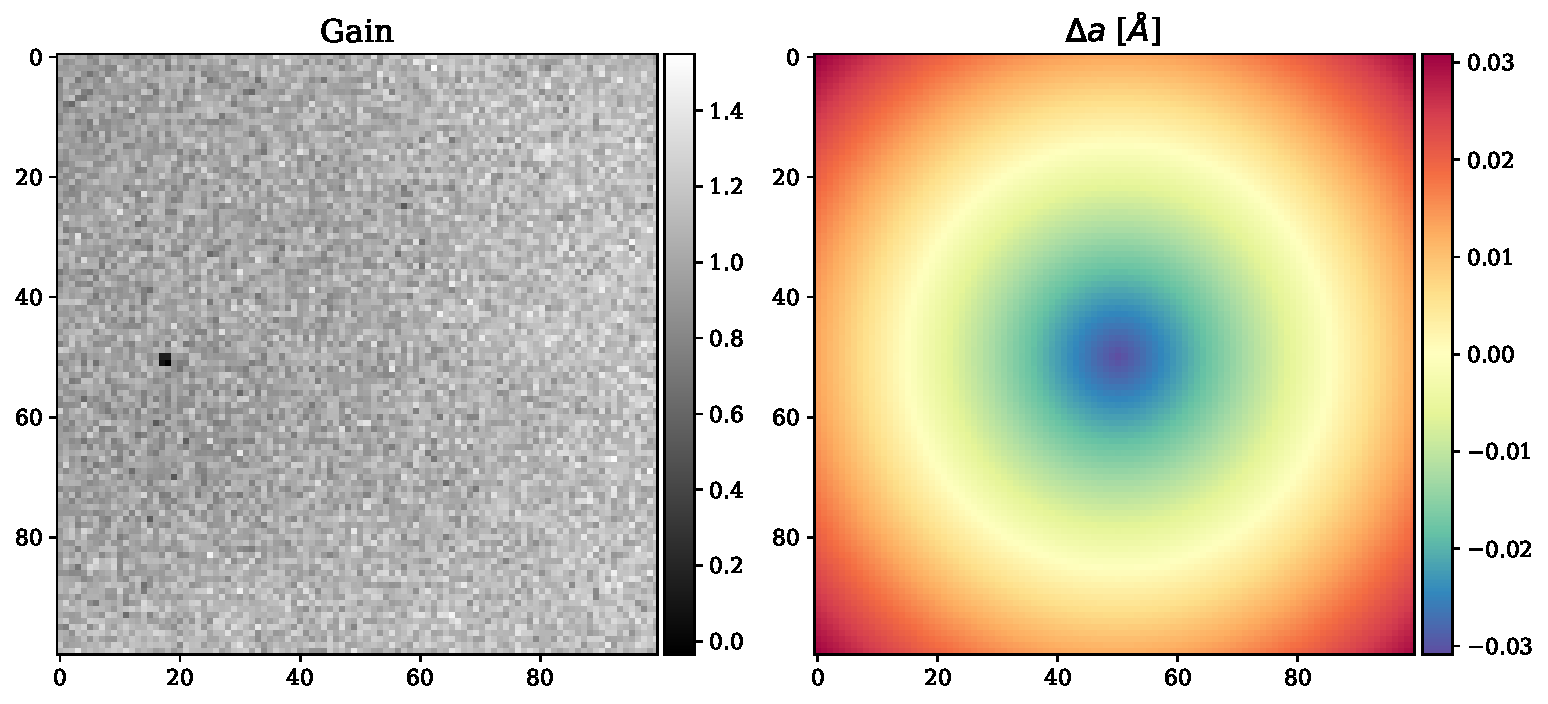
\includegraphics[width=\textwidth]{figures/EtalonPaper/Gain_Da_Inputs.pdf}
    \end{minipage}\hfill
    \begin{minipage}[c]{0.47\textwidth}
        \caption{
            Input maps introduced when simulating the observations. The top panel represents the gain generated as white Gaussian noise, with values ranging from 0.8 to 1.2. A dust speck was introduced by creating a group of four pixels with low values of $g=0.2$ for the gain. The bottom panel shows the spatial distribution of the defects in the etalon. The distribution follows a radial pattern starting from the center of the FoV. The defects vary from $0\,\%$ deviation to up to $5\times 10 ^{-4}\,\%$, which corresponds to a shift of 3~pm. Both possible directions for the deviations have been considered. The sign of the deviation is negative at the very center, which introduces a redshift, while it is positive at the corners, causing a shift of the profile into the blue.
        } \label{fig_etalon_corr: Inputs}
    \end{minipage}
    \end{figure}




\section{Sunspot observation simulation.}